\documentclass[titlepage]{article}
\usepackage[left=2.54cm,top=2.54cm,right=2.54cm,nohead]{geometry}
\usepackage{graphicx}
\setlength{\parskip}{2mm}
\title{User Manual for OGSAS}
\author{Group 22 \\
\\
Yubin Kim (y12kim, 20239608) \\
Daniel Burstyn (dmbursty, 20206120) \\
Derek Thurn (dthurn, 20228984) \\
Nathaniel Flath (nflath, 20252804)
\\
\\for Divya Nair}
\renewcommand{\thefigure}{\thesection.\arabic{figure}}

\begin{document}
\maketitle
\newpage
\tableofcontents
\newpage
\listoffigures
\newpage

% Max does overall formatting and stuff.
\section{Introduction}
\subsection{Outline}
% Max

This is the user manual for the OGSAS system used for Graduate Studies applications to the David R. Cheriton School of Computer Science. In Section~\ref{tFirstRun} below, you can view a brief sample run through the OGSAS system, which should serve to introduce you to the capabilities of this software. Later, in Section~\ref{tBasic}, you will find an outline of the basic use cases for the system---along with full diagrams. Finally, in Section~\ref{tAdvanced}, this user manual outlines the advanced features of the OGSAS system.

\subsection{Product Overview}
% Yubin
OGSAS is the first attempt to convert the previous paper-based graduate
application system to an online electronic system. Users can log on to the
system using their UWDir
credentials. Once logged on to the system, the user can perform various tasks
depending on their role; applicants fill out supplementary forms, faculty
members can view and comment on various applications etc.
Currently, OGSAS is limited to handling the graduate applications of David R.
Cheriton School of Computer Science only.

\subsection{First Sample Run}
 \label{tFirstRun}
%Nathan
As an example, let us walk you through searching for a circulated application by
student ID and accepting that application.
\begin{enumerate}
\item From the main page, click the \textbf{\textsf{Search Applications}} link.
\item Enter the student ID, as shown in Figure~\ref{nSID}.
  \begin{figure}[h!]
    \begin{center}
      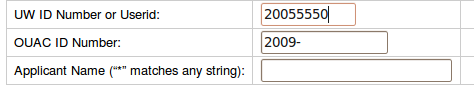
\includegraphics[width=13cm]{nsid.png}
    \end{center}
    \caption{Student ID entered}
    \label{nSID}
  \end{figure}
\item Press the \textbf{\textsf{Enter}} key when the cursor is still in the \textbf{\textsf{UW ID Number or User ID}} Field.  You will be taken to the correct application.
\item Click the Checklist tab, as shown in Figure~\ref{nChecklist}
  \begin{figure}[h!]
    \begin{center}
      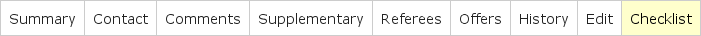
\includegraphics[width=15cm]{apptabs_checklist.png}
    \end{center}
    \caption{Checklist selected}
    \label{nChecklist}
  \end{figure}
\item Click the \textbf{\textsf{Accept this Applicant}} link, shown in Figure~\ref{nAccept}
  \begin{figure}[h!]
    \begin{center}
      
\includegraphics[width=10cm]{nAccept.png}
    \end{center}
    \caption{Accept Applicant link}
    \label{nAccept}
  \end{figure}
\end{enumerate}

Congratulations! You have now accepted an application.

\newpage
\section{Conventions}
\setcounter{figure}{0}

\subsection{User Assumptions}
\begin{itemize}
\item User is a faculty member in the David R. Cheriton School of Computer
  Science at the University of Waterloo.
\item User is the Director of Admissions at the University of Waterloo.
\item User is logged in to the OGSAS system.
\item User is familiar with the University of Waterloo graduate admissions
  process.
\item User is familiar with basic computing paradigms, such as the mouse, the
  Internet, and the keyboard.
\end{itemize}

\subsection{Notational Conventions}
\begin{itemize}
\item Serif font is for normal text.
\item \textbf{\textsf{Sans-serif Bold}} font is used for UI headings, links,
  button names etc.
\end{itemize}

\subsection{Terms}
% Max
\begin{itemize}
\item \textbf{Applicant} - A potential graduate student for the David R.
Cheriton School of Computer Science. They submit an application and are
allowed edit/view their supplementary information form and application check
list.
\item \textbf{Application Checklist} - A list of items to be completed or sent
in to UW for a complete application.
\item \textbf{Application Status} - The current state of an application. An
application initially starts as ``New" and may be assigned to other statuses
such as ``Hold", ``Initial Review", ``Circulate" at the discretion of the Admin
Staff.
\item \textbf{Reference Form} - A form that speaks of the Applicant's fitness
to be a graduate student, filled out by a referee. It is a part of the
Applicant's application.
\item \textbf{Supplementary Information Form} - A form composed of additional information
to be filled out by the Applicant.  It includes a statement about research
interests, resume, and academic background information.
\end{itemize}
\subsection{Acronyms and Abbreviations}
% Max
\begin{itemize}
\item GSO - \textbf{G}raduate \textbf{S}tudies \textbf{O}ffice
%TODO
\item OGSAS - \textbf{O}n-line \textbf{G}raduate \textbf{S}tudent \textbf{A}dmissions \textbf{S}ystem
\item OUAC - \textbf{O}ntario \textbf{U}niversities' \textbf{A}pplication
\textbf{C}entre
\item UW - \textbf{U}niversity of \textbf{W}aterloo
\item UWID - \textbf{U}niversity of \textbf{W}aterloo \textbf{ID} Number
\item UWDir - \textbf{U}niversity of \textbf{W}aterloo \textbf{Dir}ectory
\end{itemize}


\newpage
\section{Basic Use Cases}
\label{tBasic}
\setcounter{figure}{0}

\subsection{Administrative Tasks}

\subsubsection{Changing the Status of an Application}
%Yubin
\label{yChangeStatusSection}
As a member of the Admin Staff, you may wish to change the status of an
application to reflect its various states. To change the status of an
application:

\begin{figure}[h!]
  \begin{center}
  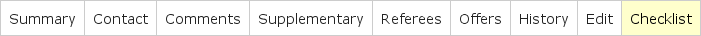
\includegraphics[width=13cm]{apptabs_checklist.png}
  \end{center}
  \caption{Checklist selected}
  \label{yChecklist}
\end{figure}

\begin{enumerate}
\item After navigating to the appropriate application, click the
  \textbf{\textsf{Checklist}} tab, shown in Figure~\ref{yChecklist}.

\begin{figure}[h!]
  \begin{center}
  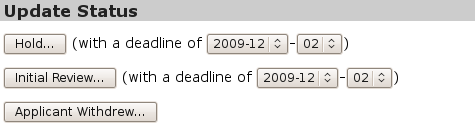
\includegraphics[width=9cm]{updatestatus.png}
  \end{center}
  \caption{Update status interface for \textbf{\textsf{Acceptance Pending}}}
  \label{yUpdate}
\end{figure}

\item Scroll down to the \textbf{\textsf{Update Status}} section, shown in
  Figure~\ref{yUpdate}.
\item Specify a deadline using the drop-down menus for the status change you
  wish to make, if appropriate.
\item Click the appropriate status button. Note that if an applicant withdraws,
  \textbf{\textsf{Update Status}} will no longer show options and will become
  an empty heading.

\begin{figure}[h!]
  \begin{center}
  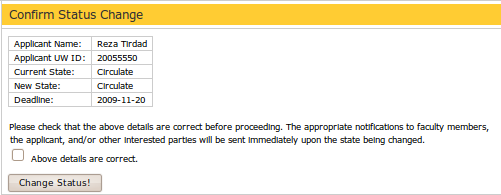
\includegraphics[width=13cm]{updatestatus_confirm.png}
  \end{center}
  \caption{Confirmation page for status changes.}
  \label{yUpdateConfirm}
\end{figure}

\item In the \textbf{\textsf{Confirm Status Change}} page as shown in
  Figure~\ref{yUpdateConfirm}, carefully review the changes. If the
  details are correct, check the box labelled \textbf{\textsf{Above details are
  correct.}} and click the \textbf{\textsf{Change Status!}} button.
\end{enumerate}

\subsubsection{Changing the Admit Term}

Changing an application's admission term (also called deferring) will remove it
from its previous term and place it in the new specified term. All of its
information, including comments and its status, will be retained.

\begin{figure}[h!]
  \begin{center}
  
\includegraphics[width=13cm]{apptabs_edit.png}
  \end{center}
  \caption{Edit selected}
  \label{yEdit}
\end{figure}

\begin{enumerate}
\item After navigating to the appropriate application, click the
  \textbf{\textsf{Edit}} tab, shown in Figure~\ref{yEdit}.

\begin{figure}[h!]
  \begin{center}
  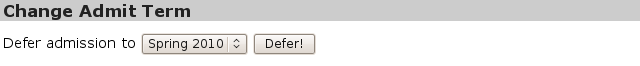
\includegraphics[width=13cm]{defer.png}
  \end{center}
  \caption{Change admit term interface}
  \label{yDefer}
\end{figure}

\item Scroll down to the \textbf{\textsf{Change Admit Term}} section, show in
  Figure~\ref{yDefer}.
\item Choose a term using the drop-down menu. This will be the term that this
  application will be deferred to.
\item Click the \textbf{\textsf{Defer!}} button.
\end{enumerate}


\subsubsection{Viewing the History of an Application}
% Thor

Periodically, it will be useful to to review the history of an application in the system to review the status changes that an application has gone through.  The system allows you to see the time at which all modifications to the status of an application occurred. This includes both internal modifications and the results of decisions by the GSO. To view the history of an application, do the following:

\begin{enumerate}
\item After navigating to the appropriate application, check the \textbf{\textsf{History}} tab, shown in Figure~\ref{tHistory}.

\begin{figure}[h!]
  \begin{center}
  
\includegraphics[width=15cm]{apptabs_history.png}
  \end{center}
  \caption{History selected}
  \label{tHistory}
\end{figure}

\item You should see two headings: \textbf{\textsf{Status History}} and \textbf{\textsf{GSO Decision History}}, and a layout of information similar to the one shown in Figure~\ref{tHistory2}.

\begin{figure}[h!]
  \begin{center}
  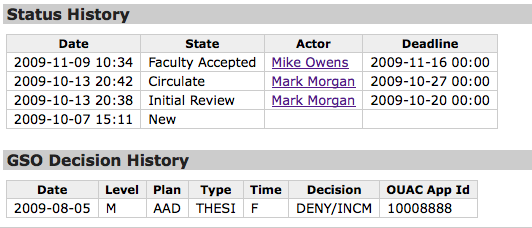
\includegraphics[width=10cm]{history_section.png}
  \end{center}
  \caption{History Section}
  \label{tHistory2}
\end{figure}

\item You can now view the date of each status change in the system, along with the actor that initiated that status change, and the deadline for that status change. You should also be able to view the record of any decisions that the GSO made about the applicant in question.

\end{enumerate}

\subsection{Faculty Tasks}

\subsubsection{Searching Applicants}
%Nathan
To search for applicants:
\begin{enumerate}
\item From the main page, click the \textbf{\textsf{Search Applications}} link.
\item Enter the field you wish to search for.  Note that only one field can be used.  The possible fields are shown in Figure~\ref{nSearchOptions}.
  \begin{figure}[h!]
    \begin{center}
      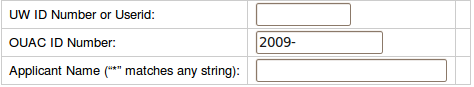
\includegraphics[width=13cm]{nsearchoptions.png}
    \end{center}
    \caption{Search options entered}
    \label{nSearchOptions}
  \end{figure}
\item Press the \textbf{\textsf{Enter}} key when the cursor is still in the field you wish to use to search.
\end{enumerate}
A list of applications matching the criteria you specified will be presented.  If only one application matched, you will be taken directly to that application.

If you want to list all applications by term and status:
\begin{enumerate}
\item From the main page, click the \textbf{\textsf{List Applications}} link.
\item Select the term and status you wish to see applications for using the drop-down lists, as shown in Figure~\ref{nListOptions}.
  \begin{figure}[h!]
    \begin{center}
      
\includegraphics[width=10cm]{nlistoptions.png}
    \end{center}
    \caption{List Application Options}
    \label{nListOptions}
  \end{figure}
\item Press the \textbf{\textsf{Search...}} button.
\end{enumerate}
You will be shown a list of all applications matching the term and status you specified.

\subsubsection{Viewing Application}
% Max
Once you have found the application you were looking for, you will be directed
to the application page.  Here you can view all the information associated
with the application.  You can view different sections of the application
using the navigation bar in Figure~\ref{mApptabs}.

\begin{figure}[h!]
  \begin{center}
  
\includegraphics[width=13cm]{apptabs.png}
  \end{center}
  \caption{Navigation Bar}
  \label{mApptabs}
\end{figure}

Here is the information that each page contains:
\begin{itemize}
\item \textbf{\textsf{Summary}}
  \begin{itemize}
    \item Applicant's citizenship information
    \item Applicant's financial support
    \item Applicant's previous academic institutions
    \item Applicant's test scores
  \end{itemize}
\item \textbf{\textsf{Contact}}
  \begin{itemize}
    \item Applicant information like name, date of birth, first language
    \item Applicant's employment history
    \item Applicant's contact information
  \end{itemize}
\item \textbf{\textsf{Comments}}
  \begin{itemize}
    \item The comments other faculty members have made on this application
  \end{itemize}
\item \textbf{\textsf{Supplementary}}
  \begin{itemize}
    \item The application workflow dates
    \item Applicant's research interests and CV
    \item Applicant's academic background
  \end{itemize}
\item \textbf{\textsf{Referees}}
  \begin{itemize}
    \item Referee contact information
    \item Reference letters
    \item Reference form data
  \end{itemize}
\item \textbf{\textsf{History}}
  \begin{itemize}
    \item Status history of the application
    \item GSO decision history for the applicant
  \end{itemize}
\item \textbf{\textsf{Edit}}
  \begin{itemize}
    \item This page allows you to edit parts of the application including
    admission term, applicant research area, and make test score corrections.
    You can read below for more in depth description on how to do this.
  \end{itemize}
\item \textbf{\textsf{Checklist}}
  \begin{itemize}
    \item This page lets you view what parts of the application have been
    scanned by the coordinator and put into the system.  From here, you can
    also change the status of an application (see below for details.)
  \end{itemize}
\end{itemize}


\subsubsection{Changing your Opinion of an Application}

%Nathan
To change your opinion of an application:
\begin{enumerate}
\item After navigating to the appropriate application, check the \textbf{\textsf{Comments}} tab, shown in Figure~\ref{nComments}.
  \begin{figure}[h!]
    \begin{center}
      
\includegraphics[width=10cm]{apptabs_comments.png}
    \end{center}
    \caption{Comments selected}
    \label{nComments}
  \end{figure}
\item Specify a new opinion using the drop-down menu for the change you wish to make.  The drop-down menu is shown in Figure~\ref{nChangeOpinion}
  \begin{figure}[h!]
    \begin{center}
      
\includegraphics[width=10cm]{nAccept.png}
    \end{center}
    \caption{Change Opinion Drop-down}
    \label{nChangeOpinion}
  \end{figure}
\item Click the \textbf{\textsf{Change!}} button.
\end{enumerate}

\subsubsection{Commenting on an Application}
% Max
You can comment on a particular application if you find it necessary.  These
will only be visible to you and other faculty members.  To leave a comment,
navigate to the \textbf{\textsf{Comments}} tab on the application page, and write your
remarks in the large text box that you can see in Figure~\ref{yCommentsPage}.
Once you submit your comment, it will be timestamped and visible to all
faculty members.

\begin{figure}[h!]
  \begin{center}
    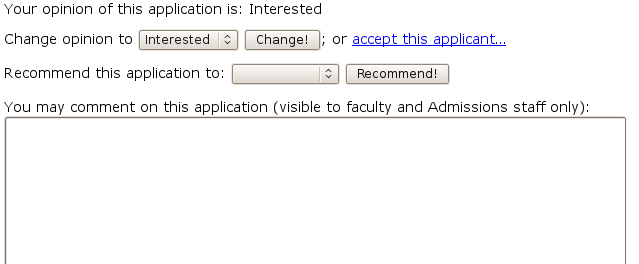
\includegraphics[width=13cm]{commentspage.png}
  \end{center}
  \caption{Comments page interface}
  \label{yCommentsPage}
\end{figure}

\subsubsection{Accepting an Application}
% Yubin
You can accept a circulating application in your capacity as a faculty member,
to indicate that you agree to supervise the applicant.

\begin{enumerate}
\item After navigating to the appropriate application, select the
  \textbf{\textsf{Comments}} tab, as shown in Figure~\ref{nComments}.
\item Click the link \textbf{\textsf{accept this applicant...}} from the
  \textbf{\textsf{Comments}} page interface shown in Figure~\ref{yCommentsPage}.

\begin{figure}[h!]
  \begin{center}
    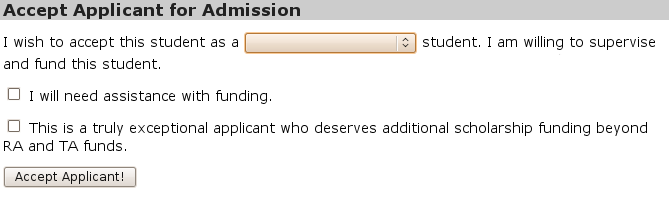
\includegraphics[width=13cm]{acceptpage.png}
  \end{center}
  \caption{Accepting an applicant}
  \label{yAcceptPage}
\end{figure}

\item In the new page (Figure~\ref{yAcceptPage}), select the student type from
  the drop-down menu.
\item If you require funding assistance, select the first check box.
\item To nominate an exceptional student for additional funding, select the
  second check box.
\item Click the \textbf{\textsf{Accept Applicant!}} button to complete the process.
\end{enumerate}

Note that, as a Director of Admissions, you may mark the application as
\textbf{\textsf{Faculty Accepted}} for another faculty member, if she agrees to
accept the student, but does not wish to go through OGSAS to indicate her
interest. Please refer to Section~\ref{yChangeStatusSection} for details.

\newpage
\section{Advanced Features}
\label{tAdvanced}
\setcounter{figure}{0}

\subsection{Administrative Tasks}

\subsubsection{Listing Authorized Users}
%Nathan
To view access roles for all authorized users:
\begin{enumerate}
\item Navigate to the \textbf{\textsf{Your Roles}} page.
\item Click the \textbf{\textsf{Show all authorized users}} link, as shown in Figure~\ref{mYourRoles}.
\end{enumerate}

You will be presented with a list of users of the system and their access roles, as shown in Figure~\ref{nroles}.

\begin{figure}[h!]
  \begin{center}
    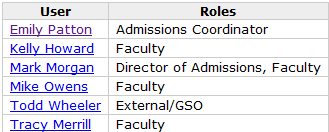
\includegraphics[width=7cm]{nroles.png}
  \end{center}
  \caption{Roles for MAT/CS David R. Cheriton School of Computer Science}
  \label{nroles}
\end{figure}

\subsubsection{Correcting Scores}
% Thor

You may wish to make corrections to the scores in the system. In the current version of the software, the two scores that can be corrected are GRE scores and TOEFL scores. Both of these are changed through the same process:

\begin{enumerate}
\item After navigating to the appropriate application, click the
  \textbf{\textsf{Edit}} tab, shown in Figure~\ref{tCorrect1}.

\begin{figure}[h!]
  \begin{center}
  
\includegraphics[width=13cm]{apptabs_edit.png}
  \end{center}
  \caption{Edit selected}
  \label{tCorrect1}
\end{figure}

\item Scroll down on the page. Near the bottom, you should see a box similar to the one shown in Figure~\ref{tCorrect2}.

\begin{figure}[h!]
  \begin{center}
  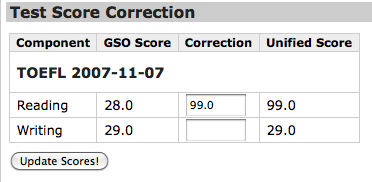
\includegraphics[width=6.5cm]{correct_scores.png}
  \end{center}
  \caption{The correct scores box}
  \label{tCorrect2}
\end{figure}

\item At this time, you can enter new values for the test scores that this applicant requires. Enter the new scores in the text boxes.
\item  When you are satisfied with the new score values, press the \textbf{\textsf{Update Scores!}} button

\end{enumerate}

\subsubsection{Changing an Applicant's Research Area}
% Thor

It may be the case that an applicant's desired research area needs to be
modified, either because of an error in the original application, or because
of a change in circumstances. It should be noted that this task cannot be
handled by the Admissions Coordinator---it is specific to the Director of
Admissions because of the judgement call it may entail. The process to change
the research area for an application is as follows:

\begin{enumerate}
\item After navigating to the appropriate application, click the
  \textbf{\textsf{Edit}} tab, shown in Figure~\ref{tResearch1}.

\begin{figure}[h!]
  \begin{center}
  
\includegraphics[width=13cm]{apptabs_edit.png}
  \end{center}
  \caption{Edit selected}
  \label{tResearch1}
\end{figure}

\item Scroll down on the page. About half way down, you should see a box similar to the one shown in Figure~\ref{tResearch2}.

\begin{figure}[h!]
  \begin{center}
  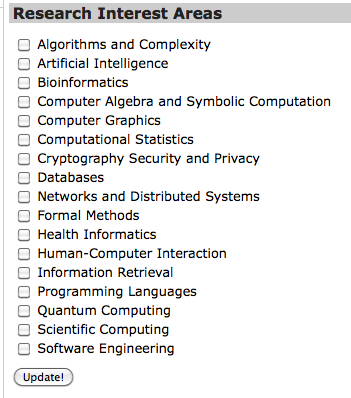
\includegraphics[width=6.5cm]{applicant_research.png}
  \end{center}
  \caption{The research interests box}
  \label{tResearch2}
\end{figure}

\item At this time, you can modify the values of the checkboxes shown to change the research areas associated with the applicant.
\item  When you are satisfied with the new research interest areas, press the \textbf{\textsf{Update!}} button

\end{enumerate}

\subsection{Faculty Tasks}

\subsubsection{Viewing Statistics}
% Thor
OGSAS allows the user to view system-wide statistics. To view statistics for the system:

\begin{enumerate}

\item Select \textbf{\textsf{View Statistics}} from the system index.
\item You should see a page like the one shown in Figure~\ref{tStats1}.

\begin{figure}[h!]
  \begin{center}
  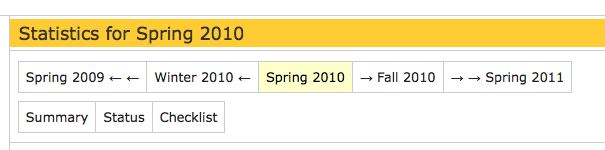
\includegraphics[width=11cm]{stats1.png}
  \end{center}
  \caption{The main screen for view statistics}
  \label{tStats1}
\end{figure}

\item You can click the name of a term at the top of the screen to view statistics for that term. Below, you can select one of \textbf{\textsf{Summary}}, \textbf{\textsf{Status}}, or \textbf{\textsf{Checklist}} to view a summary of statistics for the term, to view statistics on application statuses, or the view statistics on application checklists.

\item If you click the \textbf{\textsf{Summary}} button, you should see a summary of statistics for the system, such as the one that is shown in Figure~\ref{tStats2}. This will show you a breakdown of the applications in the system by degree level and citizenship status. You should be able to view information about the number of applicants applied, offered, and declined for admission of each degree type and citizenship status.

\begin{figure}[h!]
\  \begin{center}
  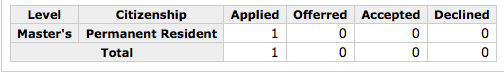
\includegraphics[width=10cm]{stats2.png}
  \end{center}
  \caption{The statistics summary screen}
  \label{tStats2}
\end{figure}

\item If you click the \textbf{\textsf{Status}} button, you should see statistics about the states of each application that the system is tracking, similar to what is shown in Figure~\ref{tStats3}. This shows how many applications in the system are in each system state.

\begin{figure}[h!]
  \begin{center}
  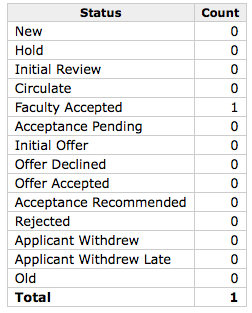
\includegraphics[width=5cm]{stats3.png}
  \end{center}
  \caption{The statistics screen for status information}
  \label{tStats3}
\end{figure}

\item Finally, if you click the \textbf{\textsf{Checklist}} button, you should see a screen similar to Figure~\ref{tStats4}. This is the statistical information about the applications in the system. It should give you information about the number of applicants that have each element of the application checklist in each state. For example, if you wanted to know what percentage of applicants are missing some information from their checklist, this would be the screen to use.

\begin{figure}[h!]
  \begin{center}
  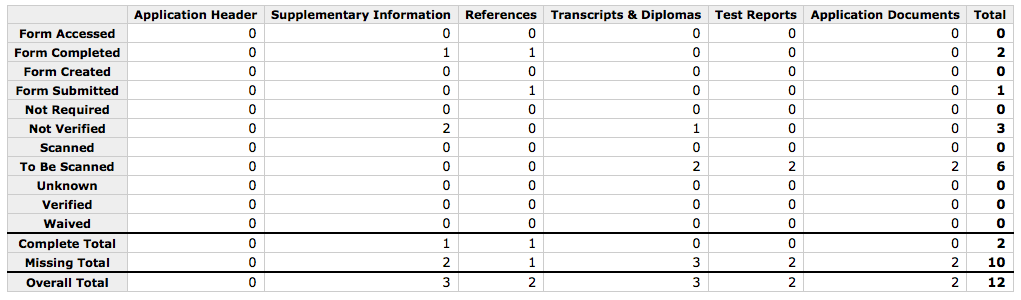
\includegraphics[width=16cm]{stats4.png}
  \end{center}
  \caption{The statistics screen for the checklist information}
  \label{tStats4}
\end{figure}

\end{enumerate}

\subsubsection{Viewing Access Roles}
% Max
From the main page, you can press the \textbf{\textsf{Your Roles}} link to view what
access authorizations you have to the system.  As the Director of admissions
the roles you see here should include DIR (Director of Admissions) and FAC
(Faculty) just like they appear in Figure~\ref{mYourRoles}.

\begin{figure}[h!]
  \begin{center}
  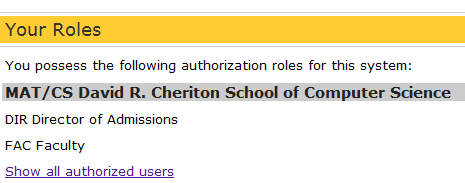
\includegraphics[width=10cm]{yourroles.png}
  \end{center}
  \caption{Your Authorization Roles}
  \label{mYourRoles}
\end{figure}

\subsubsection{Editing your Personal Info}
% Max
You, as well as all other faculty members, can update personal info through
the \textbf{\textsf{Faculty Interface}} shown in Figure~\ref{mFacultyInterface}.  From
this interface you can update your research areas, and your notification
preferences.  Clicking \textbf{\textsf{edit your research areas}} presents you with the
list of research areas in Figure~\ref{mResearchAreas} from which you can
choose one or many.  Clicking on \textbf{\textsf{edit your notification preferences}}
brings you to the notification preferences page shown in
Figure~\ref{mNotificationPreferences}.  From here, you can set what type of
notification you receive upon applications being available for review or
circulation, for comments on applications, and for student responses.  You are
also able to enable vacation mode which will turn off all notifications.

\begin{figure}[h!]
  \begin{center}
  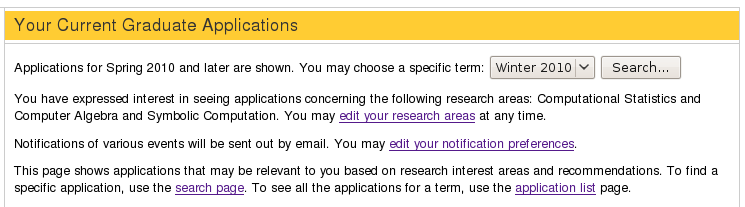
\includegraphics[width=13cm]{facultyinterface.png}
  \end{center}
  \caption{The Faculty Interface}
  \label{mFacultyInterface}
\end{figure}

\begin{figure}[h!]
  \begin{center}
  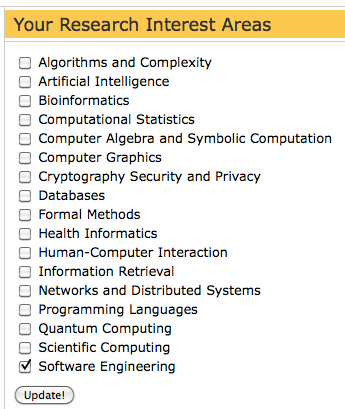
\includegraphics[width=6.5cm]{researchareas.png}
  \end{center}
  \caption{Research Areas}
  \label{mResearchAreas}
\end{figure}

\begin{figure}[h!]
  \begin{center}
  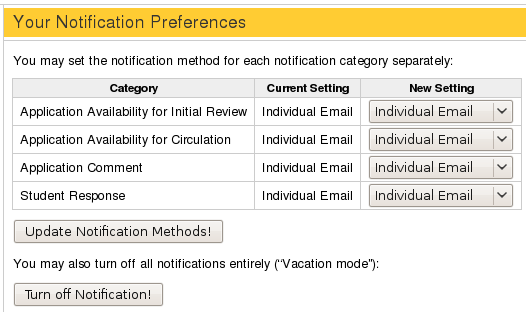
\includegraphics[width=10cm]{notificationpreferences.png}
  \end{center}
  \caption{Notification Preferences}
  \label{mNotificationPreferences}
\end{figure}

\subsubsection{Recommending an Applicant to Another Faculty Member}
% Yubin
When reading over an application, you may find that you know another faculty
member who would be a good fit with the applicant. In this situation, OGSAS
allows you to recommend an application to another faculty member.

\begin{figure}[h!]
  \begin{center}
    
\includegraphics[width=13cm]{apptabs_comments.png}
  \end{center}
  \caption{Comments tab selected}
  \label{yComments}
\end{figure}

\begin{enumerate}
  \item After navigating to the appropriate application, select the
    \textbf{\textsf{Comments}} tab, as shown in Figure~\ref{yComments}.

\begin{figure}[h!]
  \begin{center}
    
\includegraphics[width=10cm]{recommend.png}
  \end{center}
  \caption{Recommend interface}
  \label{yRecommend}
\end{figure}

  \item Find the faculty member that should receive the recommendation from
    the drop-down menu in the recommend interface. (Figure~\ref{yRecommend})
  \item Click the \textbf{\textsf{Recommend!}} button.
\end{enumerate}

\begin{figure}[h!]
  \begin{center}
    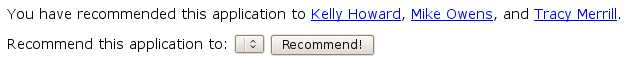
\includegraphics[width=13cm]{sentrecommend.png}
  \end{center}
  \caption{List of faculty members to whom you have recommended this
    application.}
  \label{ySentRecommend}
\end{figure}

After you have recommended an application to another faculty member, your view
of the \textbf{\textsf{Comments}} page will list them as shown in
Figure~\ref{ySentRecommend}. When these faculty members view the
\textbf{\textsf{Comments}} page, your name will appear in a list of people that have
recommend this application to them.

\newpage
\section{New Features}
\setcounter{figure}{0}

\subsection{Direct communications between Faculty and Applicant}
%Thor
\textbf{Rationale}: In the previous version of OGSAS, there was no way to communicate directly with an applicant using the system. Furthermore, communication with applicants was usually handled in a decentralized manner, which could lead to duplicated questions. A centralized means of communication would allow the University to present a consistent face to the applicant.

You may occasionally want to communicate directly with an Applicant. In the newest version of OGSAS, this is now possible. You can also view the communication of other faculty members with the applicant. To communicate with an applicant, do the following:

\begin{enumerate}
\item Go to the application page, and click on the \textbf{\textsf{Contact}} link, as shown in Figure~\ref{tCommunicate0}.

\begin{figure}[h!]
  \begin{center}
  
\includegraphics[width=13cm]{apptabs_contact.png}
  \end{center}
  \caption{Contact selected}
  \label{tCommunicate0}
\end{figure}

\item You should see the new applicant information table under the \textbf{\textsf{Applicant}} heading, as shown in Figure~\ref{tCommunicate1}. This table now shows summary information about the applicant, as well as applicant contact information.

\begin{figure}[h!]
  \begin{center}
  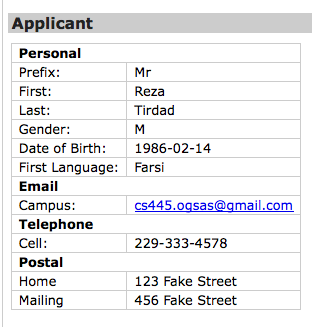
\includegraphics[width=6cm]{applicant_communication1.png}
  \end{center}
  \caption{The new applicant information table}
  \label{tCommunicate1}
\end{figure}

\item If you scroll down, you'll see the \textbf{\textsf{Contact}} heading. This is where the applicant communication functionality is based. There are two distinct sections to this screen, as shown in figure Figure~\ref{tCommunicate2}.

\item First, you should see the history of past messages in the system, with the newest messages shown first. Each message has the date attached to it, as well as the name of the individual that made the command. You can click on the name of an individual to be taken to the UWDir entry for that person.

\item Below the message history, you should see the message submit box. In this box, you can type a new message for the application. When you are done typing your message, click the \textbf{\textsf{Submit}} button. This will post your message to the application. In addition, the applicant should get an email informing them of your comments. Your message will also be visible to other faculty members. The applicant will be able to log into the system and navigate to the \textbf{\textsf{Messages}} screen, where they will be able to view messages from various professors, as well as being able to respond to messages.

\item In addition, you can modify comments that were made by you. If you click
on the \textbf{\textsf{(edit)}} link after the comment, you should see the
screen below change. The text above the text box will change to
\textbf{\textsf{Edit Message}}, and the button previously called
\textbf{\textsf{Send!}} will now be called \textbf{\textsf{Edit!}}. You should
see the text of your comments populated in the text box here. Make changes to
the text that you desire, and click \textbf{\textsf{Edit!}} when you are done.
If you want to remove your comment entirely, just press the
\textbf{\textsf{(delete)}} link after the message instead.

\begin{figure}[h!]
  \begin{center}
  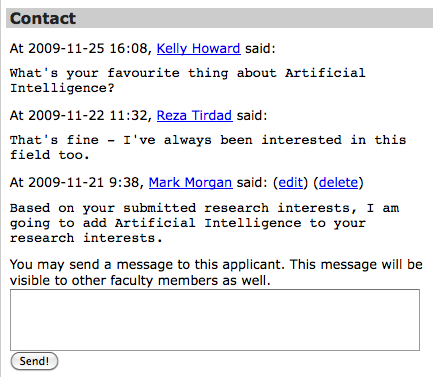
\includegraphics[width=8cm]{applicant_communication2.png}
  \end{center}
  \caption{The applicant communication area}
  \label{tCommunicate2}
\end{figure}

\end{enumerate}

\subsection{Accepting an Offer}
% Yubin
\begin{figure}[h!]
  \begin{center}
  
\includegraphics[width=13cm]{offer.png}
  \end{center}
  \caption{The main applicant interface with an offer present.}
  \label{yOffer}
\end{figure}

\textbf{Rationale}: Previously, receiving and responding to an offer was done
outside OGSAS through e-mail, and the Director of Admissions was required to
manually update the application's status.  In the newest version of OGSAS,
this is now internalized.  Once an offer is sent, there is no need for the
Director of Admissions to record the applicant's response to the offer
manually---this will be done automatically.

To accept or decline an offer, the applicant should follow these steps:

\begin{enumerate}
\item Go to the main applicant interface. If you have an offer, the screen
  should look similar to Figure~\ref{yOffer}.
\item To accept the offer:
  \begin{enumerate}
    \item Click the \textbf{\textsf{Accept Offer}} button.

\begin{figure}[h!]
  \begin{center}
  
\includegraphics[width=13cm]{acceptoffer.png}
  \end{center}
  \caption{Accept offer confirmation page.}
  \label{yAcceptOffer}
\end{figure}

    \item In the confirmation page (Figure~\ref{yAcceptOffer}), click
      \textbf{\textsf{Accept Offer}} to confirm. To think on the offer
      further, click \textbf{\textsf{Cancel}}.
  \end{enumerate}
\item To decline the offer:
  \begin{enumerate}
    \item Click the \textbf{\textsf{Decline Offer}} button.

\begin{figure}[h!]
  \begin{center}
  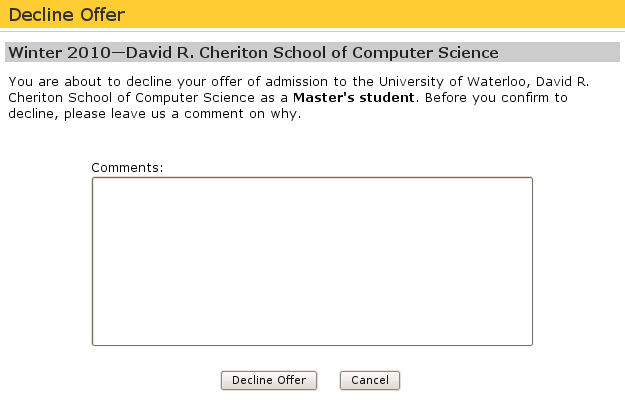
\includegraphics[width=13cm]{declineoffer.png}
  \end{center}
  \caption{The main applicant interface with an offer present.}
  \label{yDeclineOffer}
\end{figure}

    \item In the confirmation page (Figure~\ref{yDeclineOffer}), describe why
    you are declining the offer in the \textbf{\textsf{Comments:}} text box.
    \item Click \textbf{\textsf{Decline Offer}} to confirm. To think on the offer
    further, click \textbf{\textsf{Cancel}}.
  \end{enumerate}
\end{enumerate}

When an applicant accepts or declines an offer, the application's status will
automatically change accordingly, and an e-mail notification will be sent to
the Director of Admissions.

\subsection{Support for uploading scores}
\textbf{Rationale:} In the previous version of OGSAS, TOEFL and GRE scores had to be send to the Director of Admissions, who had to scan them in to the system.  In this version, this is much more optimized; the applicant can just upload the scores directly into the system.  This enhancement allows savings of time on both the applicant's and faculty's side, making for a smoother experience.

To upload applicant data such as TOEFL or GRE scores:
\begin{enumerate}
 \item The applicant will navigate to their \textbf{\textsf{Applicant Checklist}}.
 \item Click on the \textbf{\textsf{Import Data}} link, as seen in Fig~\ref{nuploadlink}.
   \begin{figure}[h!]
     \begin{center}
       
\includegraphics[width=7cm]{nuploadlink.png}
     \end{center}
     \caption{Link to Uploading Scores}
     \label{nuploadlink}
   \end{figure}
 \item Click on the \textbf{\textsf{Import}} button for the data you wish to import, or \textbf{\textsf{View Current}} to view currently imported information, as shown in Figure~\ref{nupload}.
   \begin{figure}[h!]
     \begin{center}
       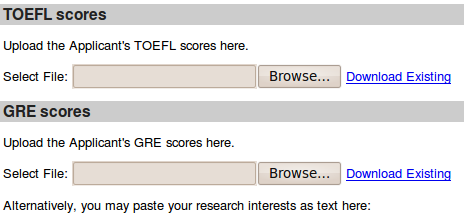
\includegraphics[width=10cm]{nscores.png}
     \end{center}
     \caption{Uploading TOEFL and GRE scores}
     \label{nupload}
   \end{figure}

 \item Once you have finished uploading data, click the \textbf{\textsf{Submit}} button, as shown in Figure~\ref{nsubmitscores}

   \begin{figure}[h!]
     \begin{center}
       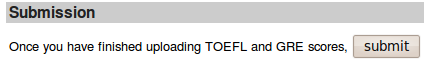
\includegraphics[width=10cm]{nsubmitscores.png}
     \end{center}
     \caption{Submitting TOEFL and GRE scores}
     \label{nsubmitscores}
   \end{figure}

\end{enumerate}

\newpage
\section{Limitations}
\setcounter{figure}{0}

\begin{itemize}
\item There is no way to search applications by research area.
\item There is no way to use multiple criteria to search for applications.
\item Statistics on gender information and other useful information are not gathered.
\item OGSAS is limited to handling the graduate applications of the David R.
Cheriton School of Computer Science only.
\end{itemize}
\end{document}

% Local Variables:
% fill-column:78
% End:
